\documentclass[]{slides}

% Begin document
\begin{document}
\printpdftrue % uncomment to hide pauses
\title[SoC design: Computer architecture - Course introduction]{\slidetitle}

% Title slide
\begin{frame} \titlepage \end{frame}

% Outline slide
%\begin{frame}{Outline} \tableofcontents \end{frame}

% ====================
% Lecturer's background
% ====================
\begin{frame}{Objective}
  \alertblue{Main objective}
  \begin{itemize}
    \item To analyse, design and successfully implement basic embedded system.
  \end{itemize}
  \alertblue{Professors}
  \begin{itemize}
    \item Dr. Isaac P\'erez Andrade (Intel).
    \item Dr. Gilberto Ochoa Ruiz (ITESM).
    \item Dr. Luis Fernando Gonz\'alez P\'erez (A2E Technologies).
  \end{itemize}
\end{frame}

% ====================
% Lecturer's background
% ====================
\begin{frame}{Lecturer's background}
\alertblue{Dr. Isaac P\'erez Andrade}
  \begin{itemize}
    \item \textbf{BSc Electronics (ITE)} - ITESM GDA - 2009.
    \item \textbf{MSc System-on-Chip} - University of Southampton, UK - 2011.
    \item \textbf{PhD Electronic Eng.} - University of Southampton, UK - 2016.
    \begin{itemize}
      \item Timing-error-tolerant iterative decoders.
      \item Digital integrated circuits design for LTE and 4G wireless communications standards.
    \end{itemize}
    \item \textbf{Digital IC Design Engineer} - Accelercomm, Southampton, UK - 2017 - 2018.
    \begin{itemize}
        \item Analysis, design and implementation of error correction code algorithms for 5G New Radio standard.
    \end{itemize}
    \item \textbf{IP logic designer} - Intel GDC - 2018 - present.
  \end{itemize}
\end{frame}

\section{Course methodology, structure, \& evaluation}
% ====================
% Course Methodology
% ====================
\subsection{Methodology}
\begin{frame}{Methodology}
\alertblue{Methodology}
\begin{itemize}
  \item Project-based learning.
  \item Self-based learning.
  \begin{itemize}
    \item Prepare before lectures by completing reading materials.
    \item Independent research.
  \end{itemize}
  \item Office hours for solving specific questions.
  \begin{itemize}
    \item Office hours are intended to provide quick guidance.
    \item Students should not expect lecturers to solve their assignments.      
  \end{itemize}
\end{itemize}
\end{frame}

% ====================
% Course structure
% ====================
\subsection{Modules}
\begin{frame}{Structure}
\begin{itemize}
  \item TE2003B System-on-Chip design comprises four modules.
  \begin{enumerate}
    \item \alertblue{Computer organisation \& architecture.}
      \begin{itemize}
        \item Prof. Isaac P\'erez Andrade - Weeks 7 - 11.
      \end{itemize}
    \item Microcontrollers.
      \begin{itemize}
        \item Prof. Gilberto Ochoa - Weeks 7 - 11.
      \end{itemize}
    \item \ac{RTOS}.
      \begin{itemize}
        \item Prof. Gilberto Ochoa - Weeks 13 - 17.
      \end{itemize}
    \item Embedded Linux.
      \begin{itemize}
        \item Prof. Luis Gonz\'alez Weeks 13 - 17.
      \end{itemize}
  \end{enumerate}
  \item Over the ten weeks of this course, you will develop a final project in which you will apply topics learned in the four modules described above.
  \item Intel will provide guidance over selected engineering topics.
\end{itemize}
\end{frame}

% ====================
% Course structure
% ====================
\subsection{Chronogram}
\begin{frame}{Structure}
\alertblue{Course chronogram}
\begin{figure}
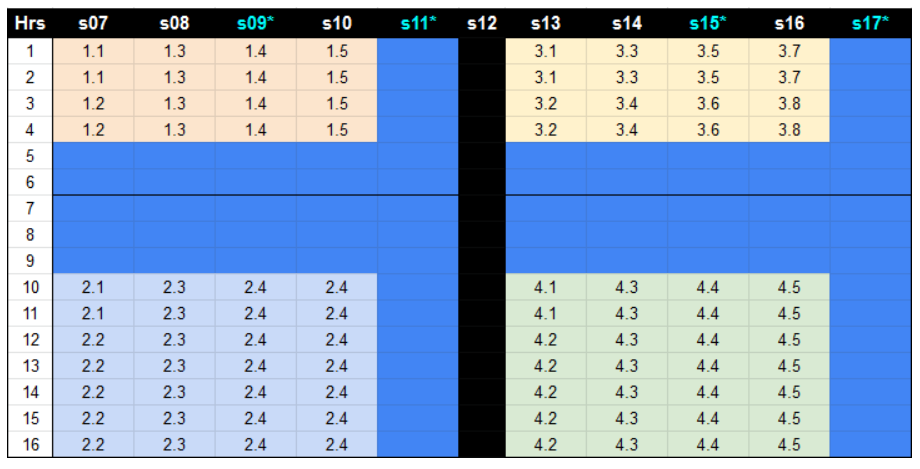
\includegraphics[scale=0.6]{Admin_Calendar}
\end{figure}
\vspace{-15pt}
\begin{itemize}
  \item Course topics are detailed in Canvas. \urlblue{https://experiencia21.tec.mx/courses/140282/modules}
\end{itemize}
\end{frame}

% ====================
% Course evaluation
% ====================
\subsection{Evaluation}
\begin{frame}{Evaluation}
\begin{figure}
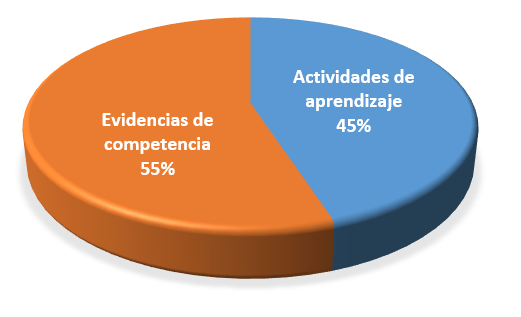
\includegraphics[scale=1]{Admin_evaluation_chart}
\end{figure}
\begin{table}[htbp]
  \begin{tabular}{l|r}
    \hline
    Modules & 45\%  \\ \hline
    Project & 55\% \\ \hline 
    \alertblue{TOTAL}                     & \alertblue{100\%} \\ \hline
  \end{tabular}
\end{table}
\end{frame}

% ====================
% Course evaluation
% ====================
\subsection{Evaluation}
\begin{frame}{Evaluation}
\alertblue{Modules evaluation}
\begin{table}[htbp]
  \begin{tabular}{l|r}
    \hline
    \alertblack{Module} & \alertblack{Weight}  \\ \hline\hline
    Computer organisation \& architecture &   15\% \\ \hline 
    Microcontrollers                      &   15\% \\ \hline    
    \acs{RTOS}                            &   10\% \\ \hline 
    Embedded Linux                        &   5\% \\ \hline
    \hline
    \alertblue{TOTAL}                     & \alertblue{45\%} \\ \hline
  \end{tabular}
\end{table}
\alertblue{Project \& evidences evaluation}
\begin{table}[htbp]
  \begin{small}
  \begin{tabular}{l|l|r}
    \hline
    \alertblack{Evidence}   & \alertblack{Competences}                                & \alertblack{Weight} \\ \hline
    Evidence 1 & STE0101.B, STE0204.B, STE0302.A            & 25\%   \\ \hline
    Evidence 2 & STE0102.B, STE0103.B, STE0303.A, SEG0702.B & 30\%   \\ \hline
    \hline
    \multicolumn{2}{r|}{\alertblue{TOTAL}}                  & \alertblue{55\%} \\ \hline
  \end{tabular}
  \end{small}
\end{table}

\end{frame}

% ====================
% Course competences
% ====================
\subsection{Competences}
\begin{frame}{Competences}
  \begin{itemize}
    \item \alertblue{STE0101B.} Modela sistemas embebidos con capacidad de interacción que dan solución a una problemática determinada.
    \item \alertblue{STE0102B.} Implementa sistemas embebidos considerando especificaciones y restricciones del entorno.
    \item \alertblue{STE0103B.} Valida el funcionamiento de sistemas embebidos tomando en cuenta la eficiencia, costos y estándares.
    \item \alertblue{STE0204B.} Elige la unidad de procesamiento acorde a requerimientos.
    \item \alertblue{STE0302B.} Selecciona el protocolo de comunicación de acuerdo a su aplicación.
    \item \alertblue{STE0303A.} Genera la interacción inteligente entre una unidad de procesamiento y sus periféricos.
    \item \alertblue{SEG0702B.} Evalúa diversas tecnologías, con apertura a la búsqueda e implementación de alternativas relevantes en la transformación de la práctica profesional.
  \end{itemize}
\end{frame}

% ====================
% Course contents
% ====================
\section{Computer organisation \& architecture contents}
\begin{frame}{Computer organisation \& architecture contents}
  \begin{enumerate}
    \item Instruction set architecture.
    \item Computer arithmetic.
    \item Processor: Datapath and control.
    \item Pipeline.
    \item Memory hierarchy and \ac{IO} interfaces.
  \end{enumerate}
\end{frame}

% ====================
% Course policies
% ====================
\section{Course policies}
\begin{frame}{Policies}
\alertblue{Web conference lectures}
\begin{itemize}
  \item Just as in face-to-face lectures, our behaviour shall be based on discipline, responsibility and respect.
  \item Lectures shall commence at 07:10 and end at 08:50 hours.
  \item Students are encouraged to join the zoom session on time.
  \item Students \alertred{must} have their webcam on during the lecture.
  \item Lectures will be recorded. Please remind your lecturer if you notice the lecture is not being recorded.
  \item Adhering to Tecn\'ologico de Monterrey ethics code, students pledge that their behaviour shall be ruled by academic honesty.
\end{itemize}
\end{frame}

% ====================
% Coursework and assignments
% ====================
\begin{frame}{Policies}
\alertblue{Coursework and assignments}
\begin{itemize}
  \item For individual assignments, students are encouraged to discuss ideas with other students. 
  However, it is expected that each student submits their own individual and original work.
  \item Students should not submit work from external sources such as websites, books or other students.
  \item For group assignments, the policy for individual assignments apply. Moreover, students must
disclose the collaboration percentage of each team member.
  \item For both individual and group assignments, \alertred{if there's evidence of students submitting other work than their own, the involved students will automatically fail the assignment}.
\end{itemize}
\end{frame}

% ====================
% Coursework and assignments
% ====================
\begin{frame}{Policies}
\alertblue{Coursework and assignments}
\begin{itemize}
  \item \alertred{Late submissions will not be tolerated.}
  \item \alertred{Late submissions will be automatically assigned a grade of 0.}
  \item \alertred{If a submission is on time but not in the specified format, the submission will be penalised by 30\%.}
  \begin{itemize}
    \item For example, if an activity is requested to be submitted through Canvas but a student submits their work through email or Google drive, the possible maximum grade for the submission will 70.
  \end{itemize}
\end{itemize}
\end{frame}

% ====================
% Suggested literature
% ====================
\section{Resources}
\begin{frame}{Suggested literature}
\begin{itemize}
\item J. L. Hennessy and D. A. Patterson, \emph{Computer architecture and design: The hardware and software interface - ARM edition}, Morgan Kaufmann, 2017.
\item S. L. Harris and D. M. Harris, \emph{Digital design and computer architecture - ARM edition}, Morgan Kaufmann, 2016.
\item J. Yiu, \emph{The definitive guide to ARM Cortex-M0 and Cortex-M0+ processors}, Second edition, Elsevier, 2015.
\end{itemize}
All these resources are available in \emph{Biblioteca Digital} (editions may vary).
\end{frame}

% ====================
% Contact
% ====================
\subsection{Contact information}
\begin{frame}{Contact information}
\begin{itemize}
\item Zoom 
\begin{itemize}
  \item Course (lectures) \urlblue{https://itesm.zoom.us/j/6215756089}.
  \item Personal (asesorías) \urlblue{https://itesm.zoom.us/j/7558517847}.
\end{itemize}
\item Remind: \textcolor{blue}{socgdaarq}
\item Email: \href{mailto:isaac.perez.andrade@tec.mx}{\textcolor{blue}{isaac.perez.andrade@tec.mx}}
\item Office hours (asesorías): No fixed schedule. However, we can schedule face-to-face sessions as needed, please send an email or Remind message with your request and proposed schedule at least 24 hours in advance.
\end{itemize}
\end{frame}

% ====================
% Course introduction (topic 0)
% ====================
\section{System-on-Chips}
\begin{frame}{System-on-Chips}
\alertblue{\acf{SoC}}\pauseprint
\begin{itemize}
  \item A single \acf{IC}, also known as \emph{chip}, that \emph{integrates} several subsystems and components that are part of a computing system.
\end{itemize}
  \begin{figure}
  \includegraphics[scale=0.55]{Qualcomm_snapdragon_blockdiagram}
  \label{Figure:QualcommSnapdragon}
  \vspace{-5pt}
  \caption{Qualcomm Snapdragon 865+ 5G \acs{SoC}.}
  \end{figure}
\end{frame}

% ====================
% Course introduction (topic 0)
% ====================
\begin{frame}{System-on-Chips}
\begin{itemize}
\item How do \acp{SoC} differ from the following?\pauseprint
  \begin{itemize}
    \item \acfp{uP}.\pauseprint
    \item \acfp{uC}.\pauseprint
    \item Embedded systems.\pauseprint
    \item \acfp{FPGA}.\pauseprint
    \item \acfp{ASIC}.
  \end{itemize}
  \pauseprint
\item Despite its name, this course will focus on \alertblue{embedded systems}, which are a vital part of consumer electronics.\pauseprint
\item Have a look at \urlblue{https://www.ifixit.com/Teardown} in order to observe the complexity of various consumer electronic products.
\end{itemize}
\end{frame}

\end{document}

